\chapter{ReLUSyn}
\label{relusyn}
\tool is our tool that demonstrates the \ac{RFDIA} vulnerability in DNN-based \ac{CPS}, by synthesizing attacks.
We explain our approach and algorithms for attack synthesis and present \tool, which implements the algorithms and synthesizes the models and attacks. 
We show how fully connected, feed-forward \ac{DNN}s can be formulated as \ac{MILP} models. 
We use a generic representation and describe the modeling of cost functions that are used to generate \ac{RFDIA}.
We then show how this allows us to identify critical inputs and find minimal perturbations. 
Finally, we demonstrate its efficiency in three real systems. 
We also include a section on how ReLU (the non-linear activation function) is likely to be modeled internally by MILP solvers based on Fischetti et al. \cite{fischetti2017deep}. %, who propose a 0-1 MILP model for \ac{DNN} modeling. 


\begin{figure}
	\centering
	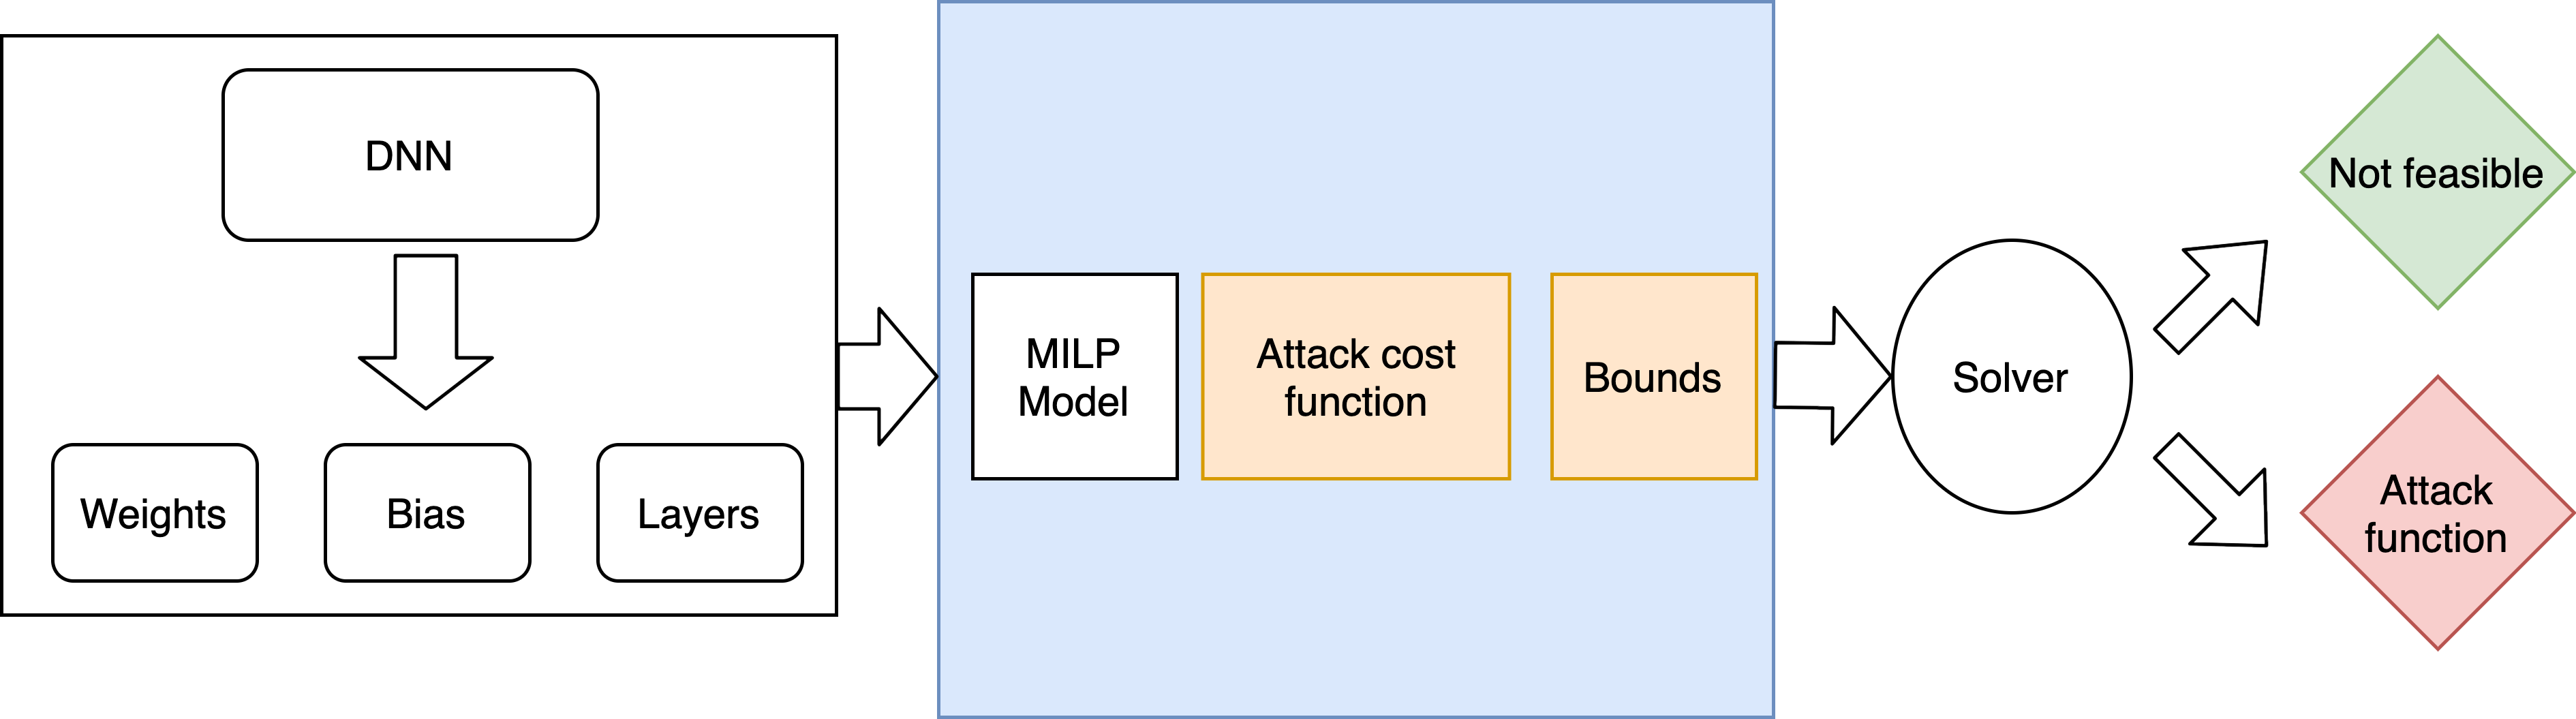
\includegraphics[scale=0.1]{Images/Methodology}
	\caption[Methodology]{The rounded boxes depict the information provided by the users and the square boxes represent the information that is required by the solver; MILP model is generated automatically and the cost functions and bounds are plugged in by the user.}
	\label{fig:methodology}
\end{figure}

\begin{figure}
	\centering
	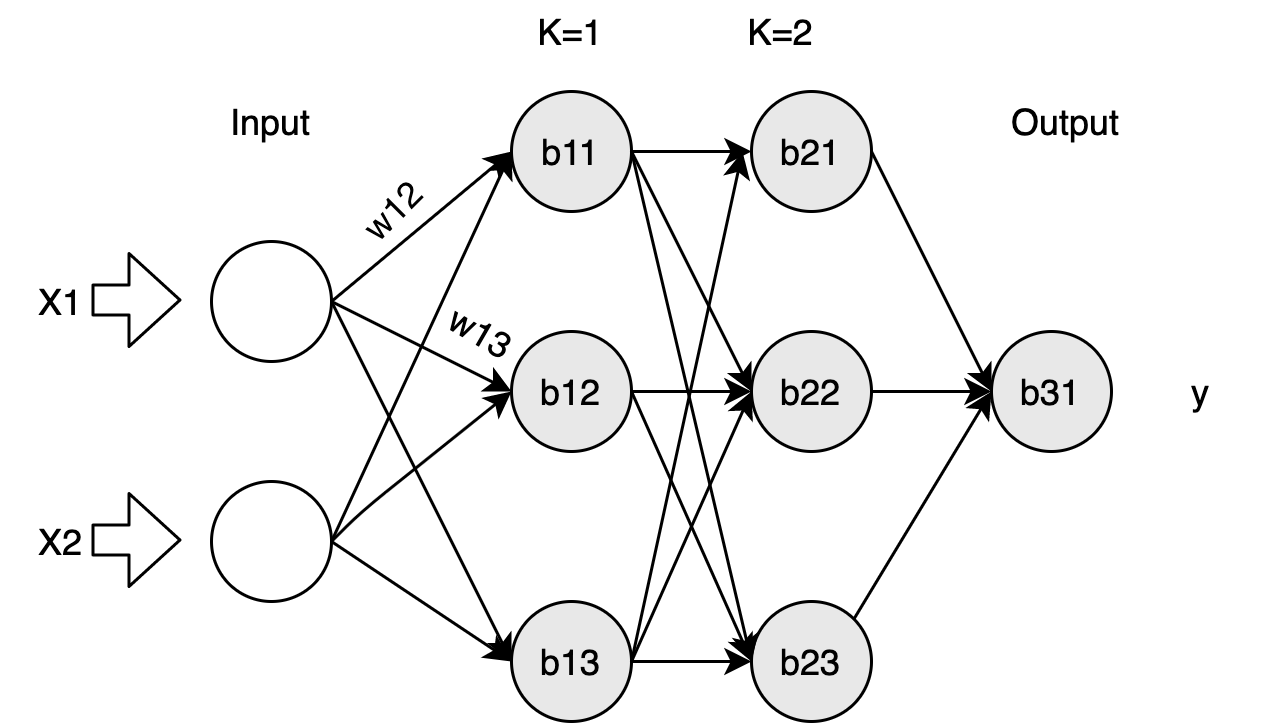
\includegraphics[width=0.7\linewidth]{Images/DNNstructure}
	\caption[DNN structure]{DNN controller structure with two hidden layers K=1,2, two inputs x1 and x2 and one output y. This is an example of a fully connected network.}
	\label{fig:dnn-controller}
\end{figure}


\section{ReLUSyn: Overview}
Figure ~\ref{fig:methodology} depicts \tool.
\begin{enumerate}
	\item \tool takes as input the DNN for a CPS controller, an optional cost function (which allows users to request particular types of attacks, which will be discussed in more detail in section~\ref{section:costfunction}), and a set of bounds indicating how much inputs can be varied without raising alarms. The bounds can be on inputs, outputs or both depending on the requirement. 
	\item \tool then produces a \ac{MILP} model for \ac{DNN}.
	\item Any solution that the  \ac{MILP} Solver finds for the model maps to a feasible attack.
	\item If there is no such solution, then no attack is possible.
\end{enumerate}

	
\section{DNN formalism}
We follow the formalism based on the general architecture presented in Chapter ~\ref{background}. 
The \ac{DNN} controller in
 Figure ~\ref{fig:dnn-controller} maps the inputs, $x1$ and $x2$ to the output $y$. 



%Formal modeling of a DNN for later use when explaining the modeling in MILP  
We represent the architecture as a function F defined as $F: X \rightarrow Y$ composed of multiple layers that maps inputs X to output Y. 
Assume \ac{DNN} composed of $K + 1$ layers, numbered 0 to K.
Layer 0 %does not really exist since it 
is the input layer, while layer K is the output.
Each layer $k$ $\epsilon$ $\{0,1,....,K\}$ consists of $n_k$ nodes (neurons).
Each neuron has a bias associated with it. 
The network is fully connected, hence each neuron from layer $k$ is an input to layer $k+1$. 
The neurons are labeled starting from $1$ to $n_k$ in the network. 
We denote each neuron by $NODE(i,k)$ which corresponds to the $ith$ node for the layer k. 

We denote the output vector of layer $k$ as $F_k(x)$.
The output for each $NODE(i,k)$ is denoted as $F_{ik}(x)$ where $i$ $\epsilon$ $\{1,....,n_k\}$ 

The output for layer 0 is represented as $F_k(0)$.
For every layer $k \geq 1$ the output vector is represented in Equation ~\ref{1}, 

\begin{equation}
\label{1}
\begin{aligned}
F_k(x) &= \upsigma(W^{k-1}x^{k-1} + b^{k-1}) \\
\end{aligned}
\end{equation}

where $W$ is the weight vector, $b$ is the bias associated with each layer, $x$ is the input to the network and $\upsigma$ represents the activation function. 
\ac{DNN}s can have various activation functions, each with different modeling capabilities. 
Two common ones are: Rectified Linear Unit (ReLU) ($f(x) = max$ (${0,x}$) as shown in Figure \ref{fig:relubreakdown} and logistic (or sigmoid) activation function $f(x)=1/(1+ exp(-e))$.
\tool focuses on ReLU,  since it is one of the commonly used activation functions according to Krizhevsky et al. \cite{10.1145/3065386} and is used in all of our example systems.

Thus, the activation function for a layer $k$ and vector $x$ is 

ReLU($x$):= $\sum_{i=1}^{n_k} e_{i}\max(0, x_{i})$ 


In this context, we can restate Equation ~\ref{1} as ~\ref{2}. 

\begin{equation}
\label{2}
\begin{aligned}
F_k(x) &= ReLU(W^{k-1}x^{k-1} + b^{k-1}) \\
\end{aligned}
\end{equation}

Since a network consists of multiple layers, the general \ac{DNN} representation is composition function where each $F_k$ represents a \ac{DNN} layer. 
\begin{equation}
\label{3}
	\begin{aligned}
	F(x) &= F_K \circ F_{K-1} \circ F_{K-2} ....... \circ F_1(x),    \\
	or \\
	F(x) &= F_K ( F_{K-1}( F_{K-2} .......  (F_1(x)))),    \\
	\end{aligned}
\end{equation}

%This ends  our \ac{DNN} formalism. In the next section we use the formalism to create a \ac{MILP} model. 

\section{MILP Model}
The non-linear ReLU activation function cannot be modeled directly by MILP solvers, so we present an equivalent formulation, which we use to identify critical inputs and find the minimum perturbations as discussed in ~\ref{problemstatement}. 
We use the Gurobi solver to do so. 

 To create a \ac{MILP} model, we study the basic scalar equation that describes the \ac{DNN} architecture where $w$ is the weight, $y$ is the input and $b$ is the bias. 

\begin{equation}
\label{4}
\begin{aligned}
x &= ReLU(w^Ty + b) \\
\end{aligned}
\end{equation}
 

We cannot apply the $f(X) = \max(0, x)$ operator directly because it is non-linear. 
As explained in Figure \ref{fig:relubreakdown}, the ReLU function can be broken in two parts, namely positive and negative parts which is termed as piecewise linear. 

In theory $f(x)$ = $Max(0,x)$ can be represented as Equation ~\ref{12}, however, \ac{MILP} does not support $if-then$ constructs because \ac{MILP} only supports logical constraints. 
Hence to model ReLU in \ac{MILP} we introduce a dummy variable $s$. 
 

\begin{equation}
\label{12}
\begin{aligned}
& if (x < 0) \\
& & then(0); \\
& else (x);	 \\
\end{aligned}
\end{equation}


Instead, we can rewrite the equation given above as follows:

\begin{equation}
\label{5}
\begin{aligned}
w^Ty + b = x - s, x \geq 0, s \geq 0 \\
\end{aligned}
\end{equation}

%The reason we represent it as in Equation ~\ref{5} is to first separate the equation from its non-linear component;  ReLU activation function is the non-linear part of Equation ~\ref{4}.
The addition of variable $s$ in Equation ~\ref{5} translates the ReLU activation function to a linear representation.
We make this division so that we can reason about the non-linear activation function separately from the actual equation. 
%We cannot directly represent the non-linear formulation as a direct representation of $x$ $>$/$<$ $0$ because that level of expressiveness is not available in a \ac{MILP}  formulation. 
%\ac{MILP} allows us to model implications but not $if$ statements. 



 To implement the piece-wise linear behavior, we define an activation variable $ac$ that imposes the logical implications. 
The choice to use different symbols was made in the interest of clarity. 
The equation in this rewritten form is linear, and it does model ReLU functionality  accurately as $x$ will always be non-negative. 

Modern MILP solvers can handle these constraints directly.

\begin{equation}
\label{6}
\begin{aligned}
ac =  1 \rightarrow x \leq 0  \\
ac =  0 \rightarrow s \leq 0  \\
ac \in \{0,1\} \\
\end{aligned}
\end{equation}

The $x \leq 0$ constraint in conjunction with $x \geq 0$ forces $x$ to zero. The other case forces $s$ to be zero.
This opens the door for a formulation that leads to unique solutions for $x$ and $s$ while enforcing the constraint $x \geq 0$.
The uniqueness may be achieved by adding a regularization term in the objective function that encourages most entries in $ac$ to be zero.
Extending this scalar example to the DNN case leads to a \ac{MILP} model of the form shown below. 


We have divided our \ac{MILP} model in three main parts. 


Equation ~\ref{7} represents the cost functions that are to be minimized or maximized.
These cost functions are different for different applications and depends on our goal; for an attack synthesis application minimization of input deviations is the goal.
The equation \ref{7} is a generic representation of cost function modeling. 
We explain our cost function in more details in \ref{section:costfunction} for \ac{RFDIA} attack synthesis. 

\begin{equation}
\label{7}
\begin{aligned}
& \underset{}{\text{min/max}}
& &  \sum_{k=0}^{K} \sum_{i=i}^{n_k}F_{jk}(x)   + \sum_{k=0}^{K} \sum_{i=i}^{n_k}F_{jk}(z)  \\
\end{aligned}
\end{equation}
%ReLU


Equations ~\ref{8} represents the ReLU modeling for each layer in the network. 
We showed in Equation~\ref{6} how we can represent ReLU units as a set of linear constraints in \ac{MILP} solvers. 
To model the constraints, we use the formalism from Equation \ref{5} where we introduce the variable $s$ to accommodate the non-linearity using linear representations as explained in \ref{6}. 
We expand on it and apply it to all the layers in the modeling.   
 
ReLU constraints
\begin{equation}
\label{8}
\begin{aligned}
& \text{subject to} & &  \sum_{j=0}^{n_k} w_{ij}^{k-1}x_{j}^{k-1} + b_i^{k-1} = x_i^k - s_i^k  \\
& & & x_i^k \geq 0, \\
& & & s_i^k \geq 0 \\
& & & ac_i^k  \epsilon  \{0,1\} \\
& & & ac_i^k  =  1 \rightarrow  x_i^k \leq 0  \\
& & & ac_i^k =  0 \rightarrow s_i^k  \leq 0   \\
\end{aligned}
\end{equation}

Equations ~\ref{9} add lower bounds ($lb$) and upper bounds ($up$) in the  model for different variables that we will  require to add limits to our search space. 
These bounds are for the input and the output layers, all other layers are unbounded and will be 0 and $+\infty$ respectively. 
 
Upper and lower bounds for range analysis are as follows.
%Lower and upper bounds on the model
\begin{equation}
\label{9}
\begin{aligned}
& & & lb \geq x_i^k \geq up, \\
& & &  lb \geq s_i^k \geq up \\
\end{aligned}
\end{equation}








Our MILP modeling applies the $f(x) = \max(0, x)$ operation directly to the output of layers because our MILP solver linearizes this internally when solving the model.





\begin{figure}
	\centering
	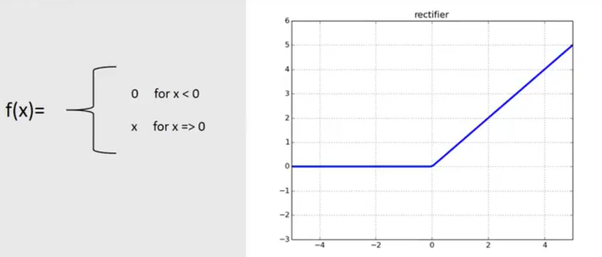
\includegraphics[width=0.7\linewidth]{Images/ReLUbreakdown}
	\caption{ReLU can be broken down into two linear units as shown in the figure for x $<$ 0 and x $\geq$ 0. This allows us to easily map the DNN equations in MILP models by breaking down the non-linearity inducing function.}
	\label{fig:relubreakdown}
\end{figure}

\section{Building the model}
\label{section:attacks}

% \tool contains automated attack synthesizers for the Artificial Pancreas System, Aircraft Collision Avoidance systems ACAS Xu and Horizontal CAS. 
 %We will continue using the \ac{APS} shown in \label{fig:toyaps} to illustrate \tool's functionality. 
%The \ac{APS} consists of two sensor inputs that determine the amount of insulin to inject at some time $t$. 
\begin{figure}
	\centering
	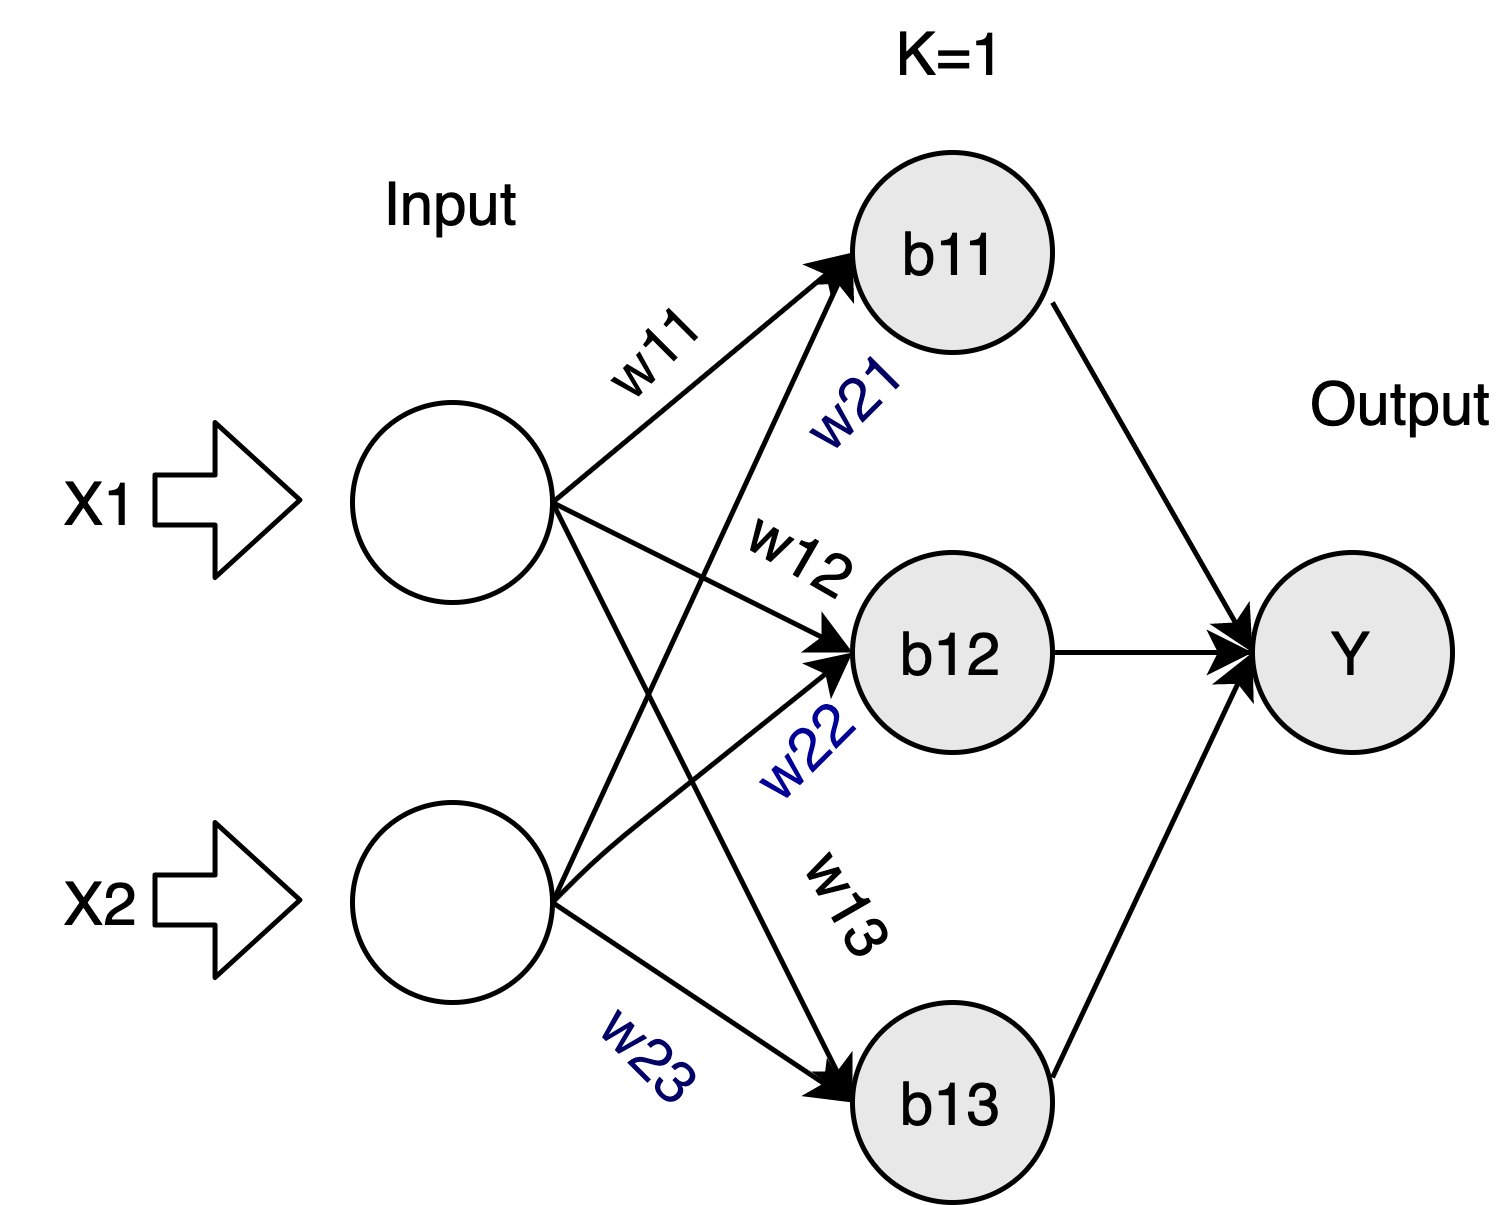
\includegraphics[width=0.7\linewidth]{Images/ToyAPS}
	\caption[APS]{APS that takes in two inputs which we consider as the sensor values from the human. It predicts the amount of insulin to be injected at some time based on the sensor inputs.}
	\label{fig:toyaps}
\end{figure}


\begin{algorithm}
	%\DontPrintSemicolon % Some LaTeX compilers require you to use \dontprintsemicolon    instead
	\KwIn{weight matrices, bias vectors, num\_layers, num\_neurons}
	\KwOut{input, layer\_output, ReLU\_output,}
	Take the weight, bias, number of layers, and the number of neurons per layer. \\
	
	\textbf{Model}, \linebreak
	%\renewcommand{\labelenumi}{(\Roman{enumi})}
	%\begin{enumerate}[noitemsep,nolistsep]
	%\item
	(I) For every layer $k$ (with weight matrix $W_k$ and bias vector $b_k$), $output_k = W_k * input_k + b_k$
	\linebreak
	%\item 
	(II) Apply activation function to every layer's output,
	\linebreak
	Constraints: $ReLU\_output_k = max(0, output_k)$ (component-wise) \
	\linebreak
	The final layer's rectified output is the DNN output.
	
	\caption{Modeling neural network in MILP}
	\label{algo:b}
\end{algorithm}


 Algorithm ~\ref{algo:b} represents an algorithm for representing a \ac{DNN} as a \ac{MILP} model. 
This converts the neural network structure into a set of linear equations that can be mapped directly into a back-end MILP solver, in our case, Gurobi. 

The DNN input for $k+1$ is the output of the $k$ layer as shown in Algorithm  ~\ref{algo:b}. 
The $inputs$ to the  Algorithm ~\ref{algo:b} is the \ac{DNN} architecture. 
The $output$ is a \ac{MILP} model that can be solved using our backend solver Gurobi. 
We use the \ac{DNN} formalism described above to map it to a \ac{MILP} model using Algorithm ~\ref{algo:b}.
%Following the same algorithm, we successfully synthesize models for \ac{APS}, \ac{ACAS-Xu}, and \ac{HCAS} within a minute. \karthik{This should go in the results section, as it is not a feature of the algorithm.}
Different applications differ only in the number of layers and nodes in each layer. 

\iffalse
Our procedure does not require an input to the DNN, as the resulting model can be solved to produce a valid input-output pair.
 Bounds can be enforced on the input variables by the user to ensure only
valid inputs are generated by the MILP solver. 
This is a positive consequence of using a constraint solving approach.
 The attacker does not need to have an input in hand when trying to compromise the system using \tool. 
 It also means that we can enumerate many such input-output pairs by repeatedly solving the model,
and adding constraints to exclude previously seen solutions.
\fi 



\begin{equation}
\label{10}
\begin{aligned}
x &= ReLU(w^Ty + b) \\
\end{aligned}
\end{equation}

\iffalse

Equation ~\ref{10} represents an \ac{APS}. 
We convert the equations above into a MILP model as shown in Algorithm ~\ref{algo:b}. 
Every layer is initially modeled as a linear equation. 
The activation function is represented as piecewise linear.
Our approach will work for any representation of a piece-wise linear function contingent on the assumption that a non-linear function can be broken down into linear components.
Since we have abstracted away the details that represent non-linearity, the future work would be representing non-linear functions as linear functions. 
 However, in our work, we focus on ReLU as explained in ~\ref{problemstatement}
\fi
\section{Modeling cost functions for attacks}
\label{section:costfunction}
%Why is modeling cost function important
Now that we have formulated the DNN as a MILP model, the next step is to add a cost or objective function corresponding to a specific kind of attack. 
This function allows the user to specify which inputs should be perturbed to generate the desired output changes.

As discussed in Chapter ~\ref{attack} the attacker's goal is to change the inputs such that it leads to an output change without triggering an alarm.
More formally, the attacker's goal is to change the output $y$ to $y'$, where $y' = y + a$ for some constant $a$. 

%She needs to find the deviations in the input that would help her to change the outputs. 
 



However, the catch here is that the inputs perturbations should be sufficiently small such to avoid detection.  


It does not consist of the cost function since the function will be different for different systems, depending on what the attacker wants to minimize and/or maximize.
In our case we are specifically demonstrating \ac{RFDIA} where the goal is to minimize the inputs deviations and/or maximize the output deviations.  
This behavior can be modeled in the objective function by introducing a new variable called $delta$ in the inputs and outputs, which is then minimized and maximized  respectively. 

Hence, the equation ~\ref{1} is represented as ~\ref{11},

\begin{align}
\label{11}
y &=  ReLU(W(x + \bigtriangleup  x ) + b)\\
\end{align}

Algorithm ~\ref{algo:c} shows how to include the cost functions for \ac{RFDIA} as a part of the MILP model. 
 
\begin{algorithm}
	%\DontPrintSemicolon % Some LaTeX compilers require you to use \dontprintsemicolon    instead
	\KwIn{input ($x$), weight matrices, bias vectors, num\_layers, num\_neurons}
	\KwOut{input\_delta ($\Delta x$), layer\_output, ReLU\_output,}
	Take the weight, bias, number of layers and number of neurons per layer. \\
	
	\textbf{Model}, \linebreak
	%\renewcommand{\labelenumi}{(\Roman{enumi})}
	%\begin{enumerate}[noitemsep,nolistsep]
	%\item
	(I) For the first layer $k = 0$ (with weight matrix $W_0$ and bias vector $b_0$), $output_0 = W_0 * (x + \Delta x) + b_k$
	\linebreak
	(II) For every subsequent layer $k \geq 1$ (with weight matrix $W_k$ and bias vector $b_k$), $output_k = W_k * input_k + b_k$
	\linebreak
	%\item 
	(III) Applying activation function to every layer's output,
	\linebreak
	Constraints: $ReLU\_output_k = max(0, output_k)$ (component-wise) \
	\linebreak
	(IV) Applying constraints to the DNN output to force the desired deviation
	\linebreak
	The final layer's rectified output is the DNN output.
	
	\textbf{Cost/Attack Function} \linebreak
	$\min |\Delta x|$
	%$Minimize $  $input\_delta$
	\caption{Modeling neural network in MILP with perturbation variables and a cost function}
	\label{algo:c}
\end{algorithm}

An attacker can choose how many inputs can be modified, assigning deltas to $0$ for those that cannot be modified. 
This is crucial in \ac{CPS} where inputs may come from different sensors and the attacker may be able to tamper with some, but not all of them.

Considering different scenarios, the attacker can minimize the values depending on which inputs they are interested in targeting with an \ac{RFDIA}. 
The \ac{RFDIA} cost function in Algorithm ~\ref{algo:c} minimizes the absolute values of the perturbations to both inputs.
%The solver can minimize the cost function despite it not being linear by introducing an extra variable for each input and adding two additional constraints per input that bound the input's value using this newly introduced variable. 



\section{Synthesizing attacks}
Once the attacker has a model and the cost function designed, the next step is to identify the critical inputs, and the desirable perturbations.
In the running example of APS, there are 74 inputs collected from two sensors every five minutes.
 The goal of the attacker is to locate the critical inputs such that they can conduct \ac{RFDIA}.
 In \ac{APS}, the attacker's goal is to maximize the output, namely the insulin to be injected into a patient, and minimize the inputs, namely the previous glucose and insulin values. 
 To do so, an attacker chooses the inputs to be perturbed, and the ranges by which they can be perturbed.  
  
 
We explain our experiments and results in the next chapter. 

